\section{Layer~4 – The Birth of Time}
\label{sec:layer4}

% ----- SUPERKRACHT -----
\begin{tcolorbox}[colback=blue!5, colframe=blue!60, title=\textbf{Superpower: The Time Weaver}]
\begin{center}
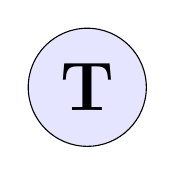
\begin{tikzpicture}
  \node[draw, circle, fill=blue!10, minimum size=1.5cm, font=\bfseries\Huge] {T};
\end{tikzpicture}
\textit{“What happens before what?”}
\end{center}
\end{tcolorbox}

Up to now, Pixel only looked at still pictures.  But the world flows.
A dust storm moves, a shadow creeps across the ground, the rover’s
metal arm bends in the wind.  To understand causality, Pixel needs a
sense of \textbf{time} – not the ticking of a clock, but the order in
which one event leads to another.

\begin{tcolorbox}[colback=yellow!5, colframe=yellow!80, title=Real‑life analogy]
A row of dominoes.  You push the first tile; it falls and pushes the
second; the second pushes the third.  The universe’s own arrow of time
is nothing more than this chain of causes.  Apeiron’s Layer~4 watches
which functional units change \emph{before} others change, and from
those observations it builds its own internal calendar.
\end{tcolorbox}

\textbf{Pixel feels the flow.}
Pixel notices that when a functional unit in the bottom‑left corner
intensifies, a unit in the top‑right corner always brightens half a
second later.  It draws an arrow: \emph{left‑bottom triggers
right‑top}.  Soon Pixel has a dynamic map of the world where past,
present, and future are defined entirely by the causal connections
between its own clusters.

\begin{figure}[ht]
\centering
\begin{tikzpicture}[
    dom/.style={rectangle, draw=black, fill=red!10, minimum width=0.8cm, minimum height=2cm},
    arrow/.style={-{Stealth}, thick}
]
\node[dom] (d1) at (0,0) {};
\node[dom] (d2) at (1.5,0) {};
\node[dom] (d3) at (3,0) {};
\node[dom, fill=gray!20] (d4) at (4.5,0) {};
\draw[arrow] (d1) -- (d2);
\draw[arrow] (d2) -- (d3);
\draw[arrow] (d3) -- (d4);
\node at (2.25,-0.8) {\small causal direction};
\end{tikzpicture}
\caption{Apeiron’s “time” is the chain of cause and effect.}
\label{fig:time}
\end{figure}

\subsection*{Why not just use a clock?}

Because the world does not tick!  Some processes are lightning fast
(a flash of lightning), others are painfully slow (the growth of a
tree).  If Pixel used an external clock, it would have to guess the
right speed for everything.  By letting time emerge from the events
themselves, Pixel always moves at exactly the right rhythm for each
situation.

\subsection*{A dash of randomness}

Pixel also adds a tiny bit of noise – deliberate randomness – to its
predictions.  Why?  Because if it always followed the exact same path,
it might get stuck in a rut.  A little exploration lets Pixel discover
new, better ways of organising its world, just like you sometimes try
a new route to school and find a shortcut.

% ----- WAT ALS...? -----
\begin{tcolorbox}[colback=orange!5, colframe=orange!60, title=\textbf{What if...?}]
What if Pixel’s internal clock runs faster than ours?  Could it see
patterns in the Martian dust that happen too slowly for a human to
ever notice?
\end{tcolorbox}